\documentclass[11pt]{article}

% ====== Packages ======
\usepackage[T1]{fontenc}
\usepackage[utf8]{inputenc}  % if you use XeLaTeX/LuaLaTeX, remove this and set fonts directly
\usepackage{lmodern}
\usepackage{microtype}
\usepackage[margin=1in]{geometry}
\usepackage{setspace}
\usepackage{xcolor}
\usepackage{graphicx}
\usepackage{subcaption}
\usepackage{booktabs}
\usepackage{siunitx}
\usepackage{amsmath,amssymb}
\usepackage{enumitem}
\usepackage{hyperref}
\usepackage[capitalize,noabbrev]{cleveref}
\usepackage{listings}
\usepackage{caption}
\usepackage{CJK}

% ====== Listings (code) style ======
\lstdefinestyle{mystyle}{
  basicstyle=\ttfamily\small,
  frame=single,
  breaklines=true,
  columns=fullflexible,
  numbers=left,
  numberstyle=\tiny,
  xleftmargin=1.5em,
  showstringspaces=false
}
\lstset{style=mystyle}

% ====== Hyperref colors ======
\hypersetup{
  colorlinks=true,
  linkcolor=blue!50!black,
  citecolor=blue!50!black,
  urlcolor=blue!50!black
}

% ====== Clever helpers ======
\newcommand{\etal}{\textit{et~al.}}
\newcommand{\ie}{i.e., }
\newcommand{\eg}{e.g., }

% ====== Project knobs (edit here to reflect final runs) ======
\newcommand{\NumRoutersA}{64}         % 4x4x4
\newcommand{\NumRoutersB}{64}         % 8x8 (2D baseline with same count)
\newcommand{\Ruby}{Garnet 3.0}
\newcommand{\SimCycles}{2{,}000{,}0}
\newcommand{\Clk}{2\,GHz}
\newcommand{\LinkW}{128\,bits}
\newcommand{\LinkLat}{1}              % ticks
\newcommand{\RouterLat}{1}            % ticks

\title{\textbf{Toward Practical 3D NoCs: Topology Design, Routing Bias, and Cost--Performance Trade-offs}\\
\large A gem5/\Ruby\ Study of 3D Mesh and Sparse-Vertical Variants}
\author{Jianan Tong \quad JiaYi Hu}
\date{\today}

\begin{document}
\maketitle

\section{Introduction}
As the demand for high-performance computing grows, Network-on-Chip (NoC) architectures are becoming essential in designing scalable, energy-efficient systems. Traditional 2D NoC topologies face limitations, particularly in large-scale systems where performance bottlenecks occur. As a result, 3D NoC topologies are gaining attention, offering reduced interconnect distances, higher bandwidth, and lower power consumption. However, 3D NoCs introduce challenges such as routing complexity, congestion, and deadlock prevention.

In this work, we explore several 3D NoC topologies that address these challenges. We focus on the design of three custom topologies and their variants, testing them against traditional mesh topologies. We evaluate their performance using different routing algorithms to analyze their effectiveness in reducing latency and maximizing throughput, while avoiding deadlocks.

The contributions of this report are as follows:
\begin{itemize}
\item The design and evaluation of novel 3D NoC topologies to improve scalability and reduce congestion.
\item A comparison of routing algorithms in terms of performance under various traffic models.
\item Simulation results demonstrating the trade-offs between topology complexity, routing efficiency, and overall system performance.
\end{itemize}

This report is organized as follows: Section 2 describes the proposed topologies. Section 3 discusses routing algorithms and deadlock avoidance. Section 4 presents the methodology and results. Section 5 concludes with findings and future directions.
\section{Topology Designs}
In this section, we describe the 3D NoC topologies explored in this study. These topologies aim to address the challenges of scalability, congestion, and deadlock in 3D NoCs. We provide an overview of their design principles, key parameters, and intended advantages. Each topology is tailored to balance performance and cost, leveraging unique structural features such as sparse vertical links, clustered hubs, or express paths to optimize routing efficiency and reduce latency.
\subsection{Mesh}

The \textbf{Mesh} topology serves as the baseline for our study, implemented in both 2D and 3D variants to provide performance benchmarks. The 2D Mesh is a standard grid where each router connects to its four immediate neighbors (North, South, East, West). The 3D Mesh extends this design into the third dimension by stacking multiple 2D layers and connecting them vertically using Through-Silicon Vias (TSVs), which enhance connectivity and reduce path lengths.

\subsection{Sparse Pillars}

One of the direct challenges of 3D NoCs is the high cost and complexity associated with dense vertical connections. To address this, we introduce the \textbf{Sparse Pillars} topology, which strategically reduces the number of vertical links while maintaining efficient inter-layer communication. The \textbf{Sparse Pillars} topology reduces the number of vertical links (TSVs) compared to the traditional 3D mesh. Instead of connecting every router to every other router in the vertical dimension, only key ``pillar" points are connected, creating a sparse network of vertical links.

\subsection{Chiplet}

To enhance the performance and scalability of 3D NoCs, we can induce a hierarchical structure like the \textbf{Chiplet} topology.
The \textbf{Chiplet} topology is a hierarchical 3D network designed to improve scalability and reduce latency in large-scale NoC systems. It divides the global network into smaller sub-units called chiplets, each containing a set of routers. These chiplets are organized in a 3D grid, with horizontal communication handled within each chiplet and vertical communication between chiplets facilitated by gateway (GW) routers.

Each chiplet connects to its neighbors via backbone links, which form the horizontal network, while the vertical connections between chiplets are made through dedicated gateways. This hierarchical structure allows for efficient intra-chiplet communication and minimizes the complexity of inter-chiplet communication.

\subsection{Cluster}

The \textbf{Cluster} topology is another hierarchical 3D network designed to optimize communication efficiency and scalability. It divides the 3D network into clusters, each containing a set of routers (Hub Routers, HBRs) that serve as the core communication points within their cluster. The network is organized in a 3D mesh with each layer consisting of multiple clusters. Each cluster is composed of four horizontal routers (HRs), which connect to a central Hub Router (HBR) that acts as the communication hub for that cluster. Vertical connections only exist between HBRs across different layers, reducing the need for extensive Through-Silicon Vias (TSVs) and improving scalability.

\section{Routing Algorithms and Deadlock Prevention}

The effectiveness of 3D NoC architectures depends critically on the routing algorithms employed to navigate packets through the network topology. We examine both minimal adaptive algorithms that prioritize shortest paths and congestion-aware mechanisms that incorporate historical network state and propose two routing strategies designed to optimize performance.

\subsection{Adaptive Minimal Routing Algorithm}

Building upon traditional table-based routing, we implement a minimal adaptive routing algorithm that dynamically selects paths based on local congestion conditions while preserving deadlock freedom through minimal path constraints.

\subsubsection{Algorithm Design}
The adaptive routing mechanism operates by first identifying all minimal paths between source and destination nodes, consistent with deterministic routing approaches. When multiple minimal alternatives exist, the algorithm evaluates congestion at candidate downstream routers by examining available virtual channel credits. The selection criterion prioritizes the outport with maximum available buffer capacity, indicating the least congested route. In cases where multiple outports exhibit identical credit levels, a round-robin arbitration policy ensures fair load distribution.

\subsubsection{Performance Characteristics}
This approach provides several key advantages for 3D NoC environments. The congestion-aware path selection effectively distributes traffic load across available minimal routes, improving overall network utilization under varying traffic conditions. Furthermore, the localized decision-making process minimizes computational overhead while providing responsive adaptation to immediate network conditions.

However, the algorithm exhibits certain limitations that may impact performance under specific scenarios. The constraint to minimal paths restricts routing flexibility when all shortest routes experience congestion, potentially leading to suboptimal load balancing. Additionally, the reliance on purely local congestion information may not capture global network state, limiting the algorithm's effectiveness in addressing system-wide traffic imbalances.

\subsection{Congestion-Aware Routing with Historical Context}

To address the limitations of purely reactive routing, we develop an enhanced algorithm that incorporates both instantaneous and historical congestion metrics for improved routing decisions in 3D mesh topologies.

\subsubsection{Mathematical Framework}
The enhanced routing algorithm computes a composite score $S_i$ for each candidate outport $i$ using the linear combination:
\begin{equation}
S_i = \alpha \cdot C_i(t) + \beta \cdot H_i(t)
\end{equation}
where $C_i(t)$ represents the instantaneous available credits, $H_i(t)$ denotes the exponentially weighted moving average (EWMA) of historical congestion, and $\alpha$, $\beta$ are weighting parameters satisfying $\alpha + \beta = 1$. The historical component evolves according to:
\begin{equation}
H_i(t) = \gamma \cdot H_i(t-1) + (1-\gamma) \cdot U_i(t-1)
\end{equation}
where $U_i(t-1)$ represents the utilization of outport $i$ in the previous time window, and $\gamma$ controls the decay rate of historical information.

\subsubsection{Stability Mechanisms}
To maintain routing stability and minimize packet reordering, the algorithm implements a path persistence mechanism. When the previously selected outport remains among the highest-scoring alternatives within a configurable threshold, it is preferred over equally-ranked alternatives. This "stickiness" property reduces routing oscillations and maintains in-order packet delivery, which is crucial for higher-level protocol efficiency.

\subsubsection{Performance}
The incorporation of historical congestion data enables more informed routing decisions that consider both current and past network conditions, leading to improved load balancing and reduced hotspot formation. The EWMA smoothing helps filter transient congestion spikes, providing more stable routing behavior compared to purely reactive approaches.

\subsection{UGAL-L (Local) Routing}

We additionally implement UGAL-L (Universal Globally-Adaptive Load-balanced, local decision; exposed as \texttt{\,--routing-algorithm=5}). UGAL-L chooses between a minimal first hop and a single non-minimal detour at the \emph{source} router using only local congestion information; all downstream routers resume minimal routing. This single-segment detour improves load balance without requiring global state.

\subsubsection{Algorithm Design}
At the source router (packets arriving from the Local port), the router constructs two candidate sets: (i) minimal outports obtained from the routing table's minimum-weight entries to the destination, and (ii) non-minimal outports consisting of all other physical directions excluding the Local port. For each set, the router picks the outport with the smallest aggregate buffer occupancy across the non-escape virtual channels, using credit counters as a proxy for congestion. If no non-minimal option exists, it defaults to minimal.

\subsubsection{Decision Rule}
UGAL-L compares the locally estimated cost of taking the best minimal outport versus the best non-minimal outport, adding a fixed detour penalty to reflect the extra distance of a misroute:
\begin{align}
\mathit{cost}_{\min} &= \mathrm{occ}(o_{\min}) \\
\mathit{cost}_{\mathrm{nonmin}} &= \mathrm{occ}(o_{\mathrm{nonmin}}) + P
\end{align}
where $\mathrm{occ}(\cdot)$ is the sum of per-VC occupancies on the outport (escape VC excluded) and $P$ is a hop-equivalent penalty. The router selects the non-minimal outport when
\begin{equation}
 \mathit{cost}_{\mathrm{nonmin}} \cdot T < \mathit{cost}_{\min},
\end{equation}
with tolerance factor $T$ (values $T{<}1$ encourage non-minimal detours). Ties are broken in favor of minimal routing. After the first hop, packets are routed minimally to their destination, which simplifies correctness and avoids persistent misrouting.

\subsubsection{Configuration and Integration}
UGAL-L is configured via two knobs: \texttt{\,--ugal-penalty} ($P$, default 2) and \texttt{\,--ugal-tol} ($T$, default 1.0). The escape VC remains strictly minimal and is excluded from congestion estimation to preserve deadlock freedom; UGAL-L engages only on adaptive VCs. Per-router statistics track the fraction of minimal vs non-minimal choices to validate that the policy activates under load.

\subsubsection{Expected Behavior}
Under uniform and hotspot traffic, UGAL-L reduces pressure on congested minimal paths by opportunistically detouring the first hop when local queues indicate imbalance, then rejoining a minimal route. This typically improves saturation throughput and tail latency while maintaining simple hardware and minimal state at intermediate routers.

\subsection{Escape Virtual Channel Mechanism}

To ensure deadlock-free operation across all routing algorithms and traffic conditions, we implement an escape virtual channel (VC) mechanism that provides guaranteed progress for packets at risk of participating in cyclic dependencies.

\subsubsection{Theoretical Foundation}
The escape VC mechanism leverages the principle that maintaining a deadlock-free subset of routing rules can prevent system-wide deadlocks, even when other VCs employ more flexible routing policies. By reserving one VC (VC$_0$) for strictly ordered routing, the system maintains a spanning tree of deadlock-free paths while allowing other VCs to exploit additional routing flexibility.

\subsubsection{Implementation Strategy}
The escape mechanism employs a breadth-first search (BFS) algorithm to precompute alternative routing trees that guarantee packet progress. When adaptive routing algorithms detect potential deadlock conditions or encounter persistent congestion, packets are dynamically migrated to the escape VC. This migration ensures continued packet advancement through the predetermined deadlock-free paths, preventing system-wide blocking conditions.
\section{Experimental Evaluation}

This section presents our comprehensive performance evaluation of the proposed 3D NoC topologies and routing algorithms. We conduct all experiments using the gem5 simulator with \Ruby\ (Garnet 3.0), employing systematic comparison across traffic patterns, topology variants, and manufacturing constraints.
\begin{figure}[th]
    \centering
    \begin{subfigure}[t]{0.45\linewidth}
        \centering
        \includegraphics[width=\linewidth]{./figs/inj_rate_vs_throughput_Mesh_XY.png}
        \caption{Throughput characteristics of the 2D mesh}
        \label{fig:mesh2d-performance}
    \end{subfigure}
    \hfill
    \begin{subfigure}[t]{0.45\linewidth}
        \centering
        \includegraphics[width=\linewidth]{./figs/inj_rate_vs_throughput_Mesh3D_XYZ.png}
        \caption{Throughput characteristics of the 3D mesh}
        \label{fig:mesh3d-performance-comparison}
    \end{subfigure}
    
    \vspace{1em}
    
    \begin{subfigure}[t]{0.45\linewidth}
        \centering
        \includegraphics[width=\linewidth]{./figs/throughput_vs_latency_Mesh_XY.png}
        \caption{Latency-throughput trade-off in the 2D mesh}
        \label{fig:mesh2d-latency-throughput}
    \end{subfigure}
    \hfill
    \begin{subfigure}[t]{0.45\linewidth}
        \centering
        \includegraphics[width=\linewidth]{./figs/throughput_vs_latency_Mesh3D_XYZ.png}
        \caption{Latency-throughput trade-off in the 3D mesh}
        \label{fig:mesh3d-latency-throughput}
    \end{subfigure}
    \caption{Comprehensive 2D versus 3D mesh comparison with equivalent router resources, demonstrating systematic advantages of three-dimensional organization.}
    \label{fig:mesh-comparison-full}
\end{figure}
\subsection{Experimental Setup and Baseline Comparison}

Our evaluation employs a standardized simulation framework with \Clk\ system clock, \LinkW\ link bandwidth, and \LinkLat\ cycle link latency. We compare \NumRoutersA\ router configurations across 2D ($8{\times}8$) and 3D ($4{\times}4{\times}4$) mesh topologies to establish performance baselines. The experiments use 2 virtual channels per network with 8-flit buffers, and evaluate three canonical traffic patterns: uniform random (global communication), transpose (hotspot stress), and nearest neighbor (spatial locality).

\subsubsection{2D versus 3D Mesh Performance}

The comparative analysis between 2D and 3D mesh topologies constitutes a fundamental evaluation for establishing the performance benefits of three-dimensional NoC architectures. Our experimental results demonstrate that 3D mesh implementations exhibit significant performance improvements across multiple evaluation metrics, providing empirical validation for the theoretical advantages of vertical integration in on-chip networks.

\textbf{Throughput Analysis:} The throughput characteristics presented in \Cref{fig:mesh-comparison-full} reveal substantial performance gains for 3D configurations. Under uniform random traffic, the 3D mesh topology achieves a saturation throughput of 0.26 packets/node/cycle compared to 0.16 packets/node/cycle for the equivalent 2D mesh, representing a 62.5\% improvement in sustained packet delivery rate. This enhancement becomes more pronounced under high injection rates, where the 3D architecture maintains stable performance while the 2D counterpart experiences throughput degradation due to network congestion.

\textbf{Latency Reduction:} The three-dimensional organization provides significant reductions in packet traversal latency through shortened communication paths. Our measurements indicate an average hop count reduction from 5.3 hops in the 2D mesh to 3.75 hops in the 3D configuration—a 29.2\% decrease in path length. This reduction directly correlates with lower zero-load latency and improved performance under light traffic conditions. The latency-throughput characteristics demonstrate that the 3D mesh maintains lower packet latency across the entire operational range, with particularly notable improvements at moderate to high injection rates.




\begin{figure}[b]
    \centering
    \begin{subfigure}[t]{0.48\linewidth}
        \centering
        \begin{center}
        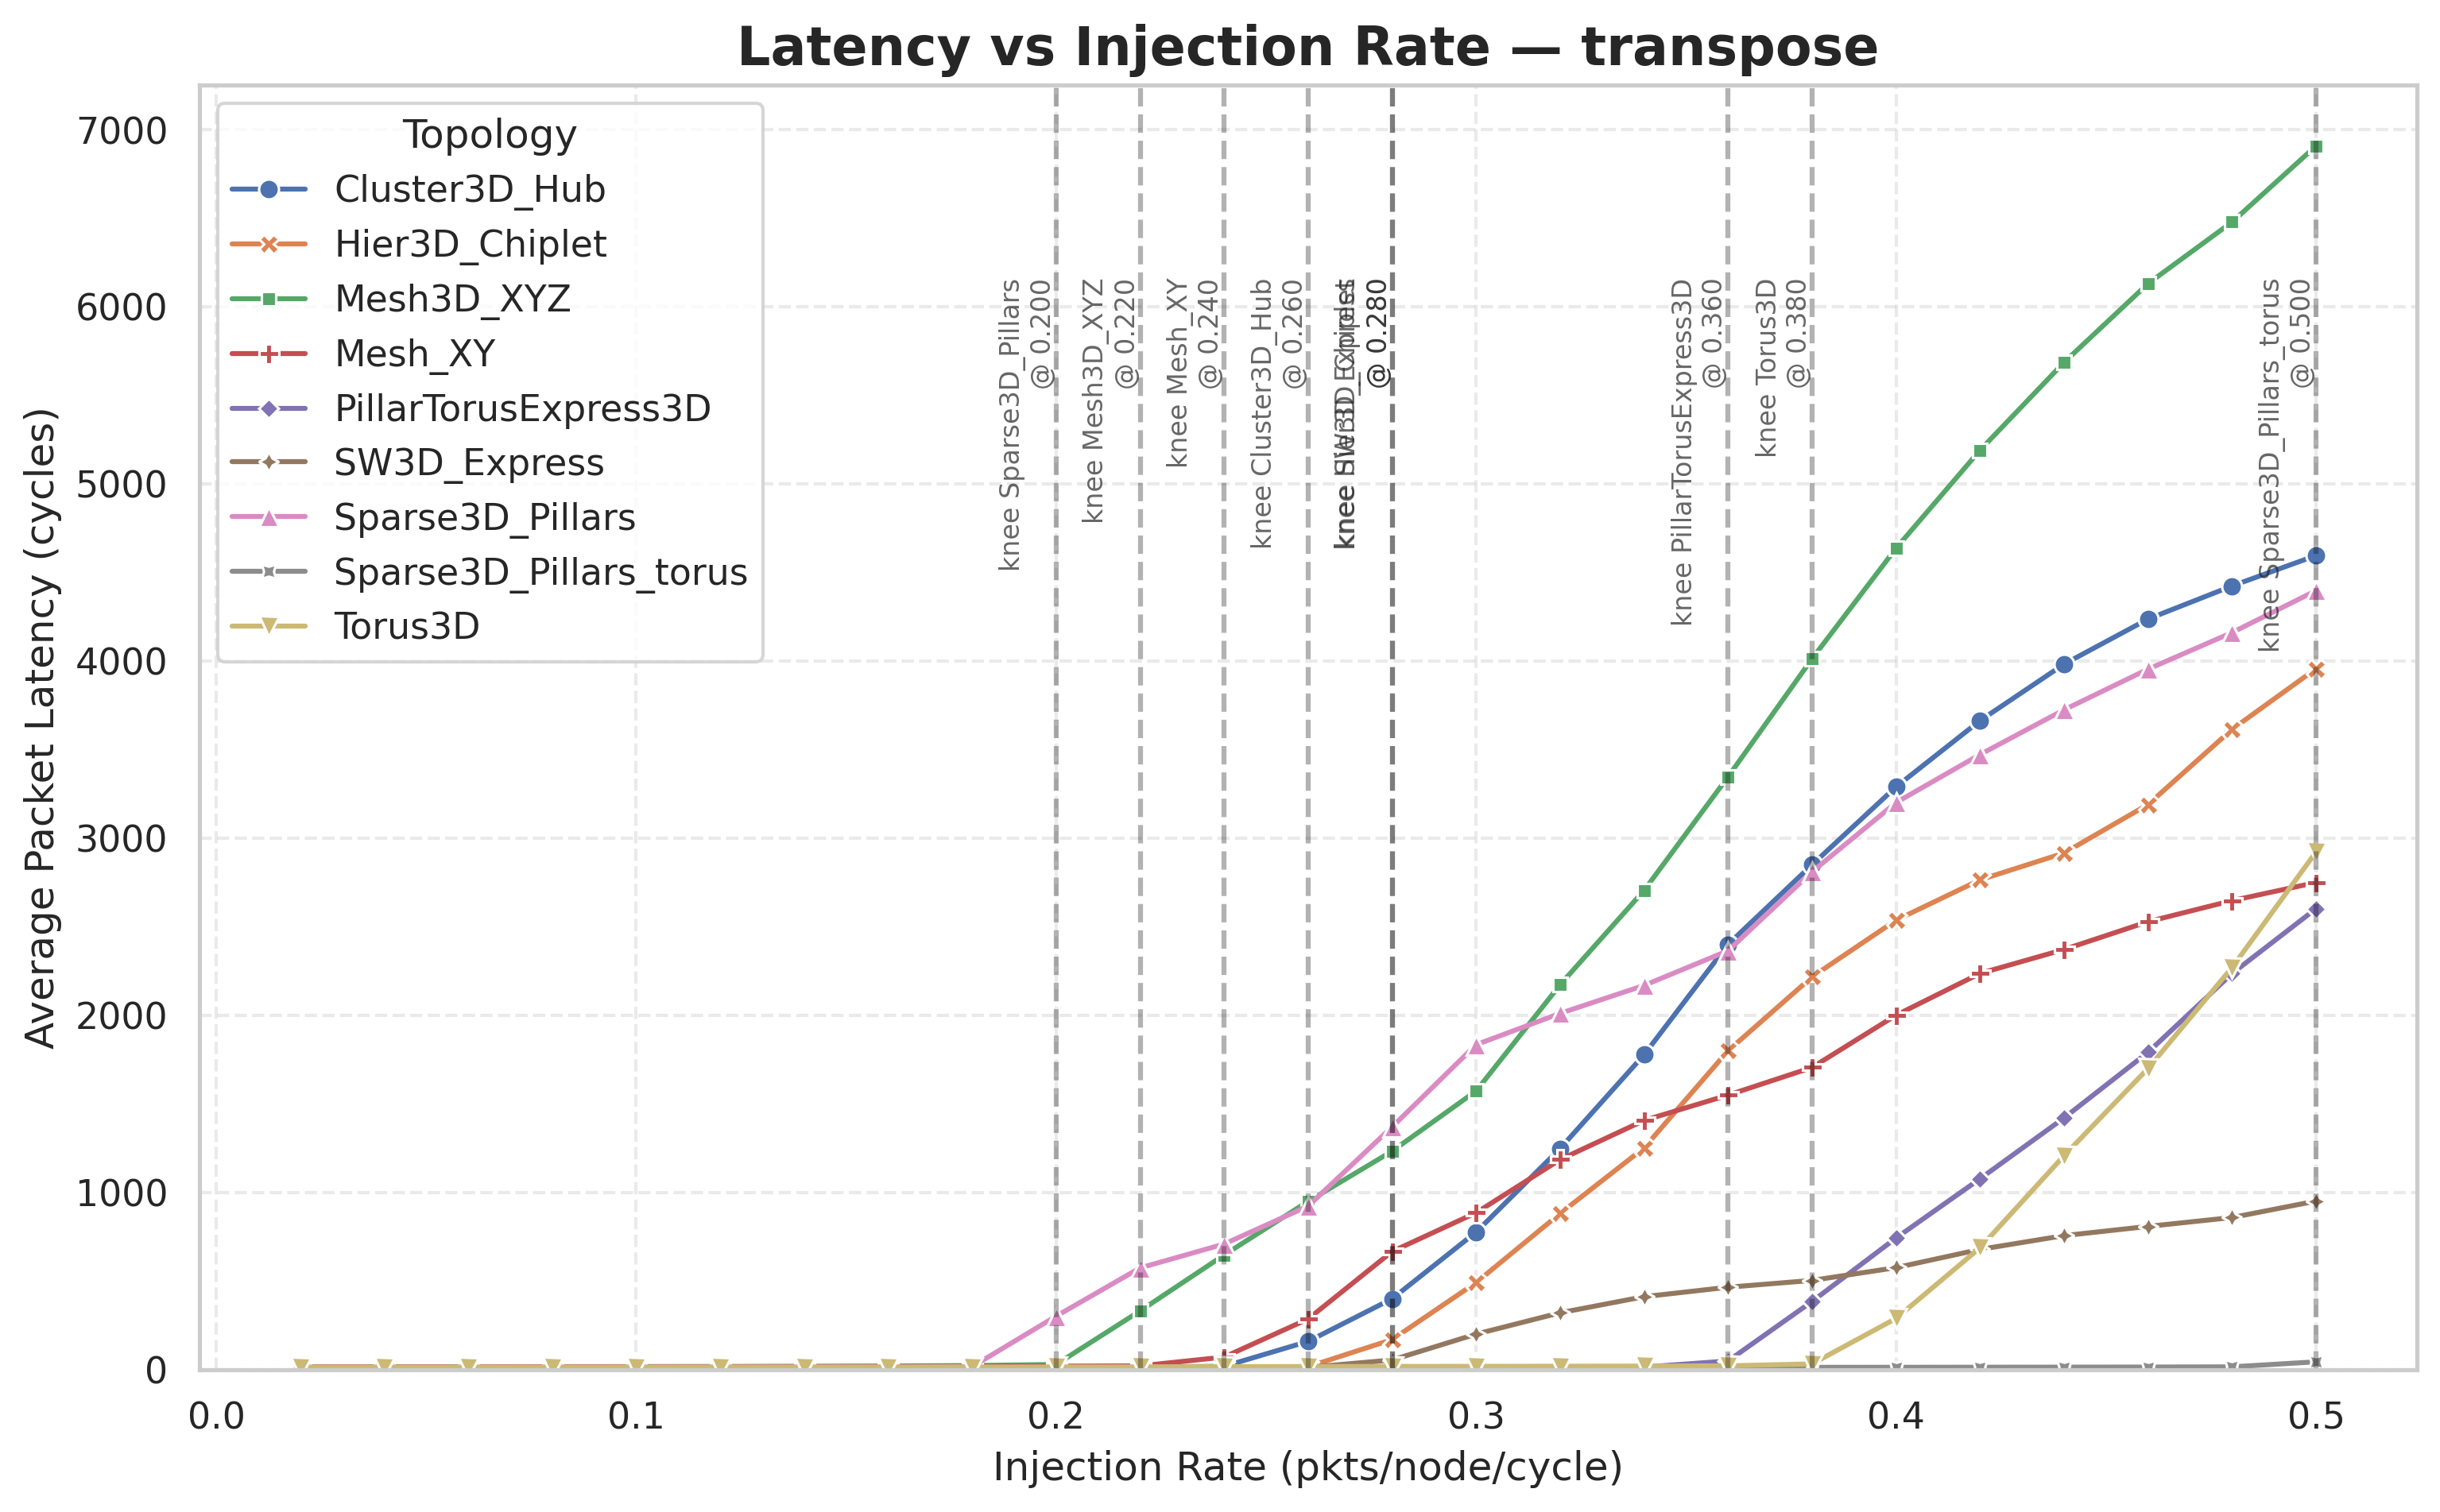
\includegraphics[width=\linewidth]{./figs/plots/latency_vs_injection_transpose.png}
        \end{center}
        \caption{Quantitative comparison of topology variants highlighting relative design advantages.}
        \label{fig:topology-efficiency-comparison}
    \end{subfigure}\hfill
    \begin{subfigure}[t]{0.48\linewidth}
        \centering
        \begin{center}
        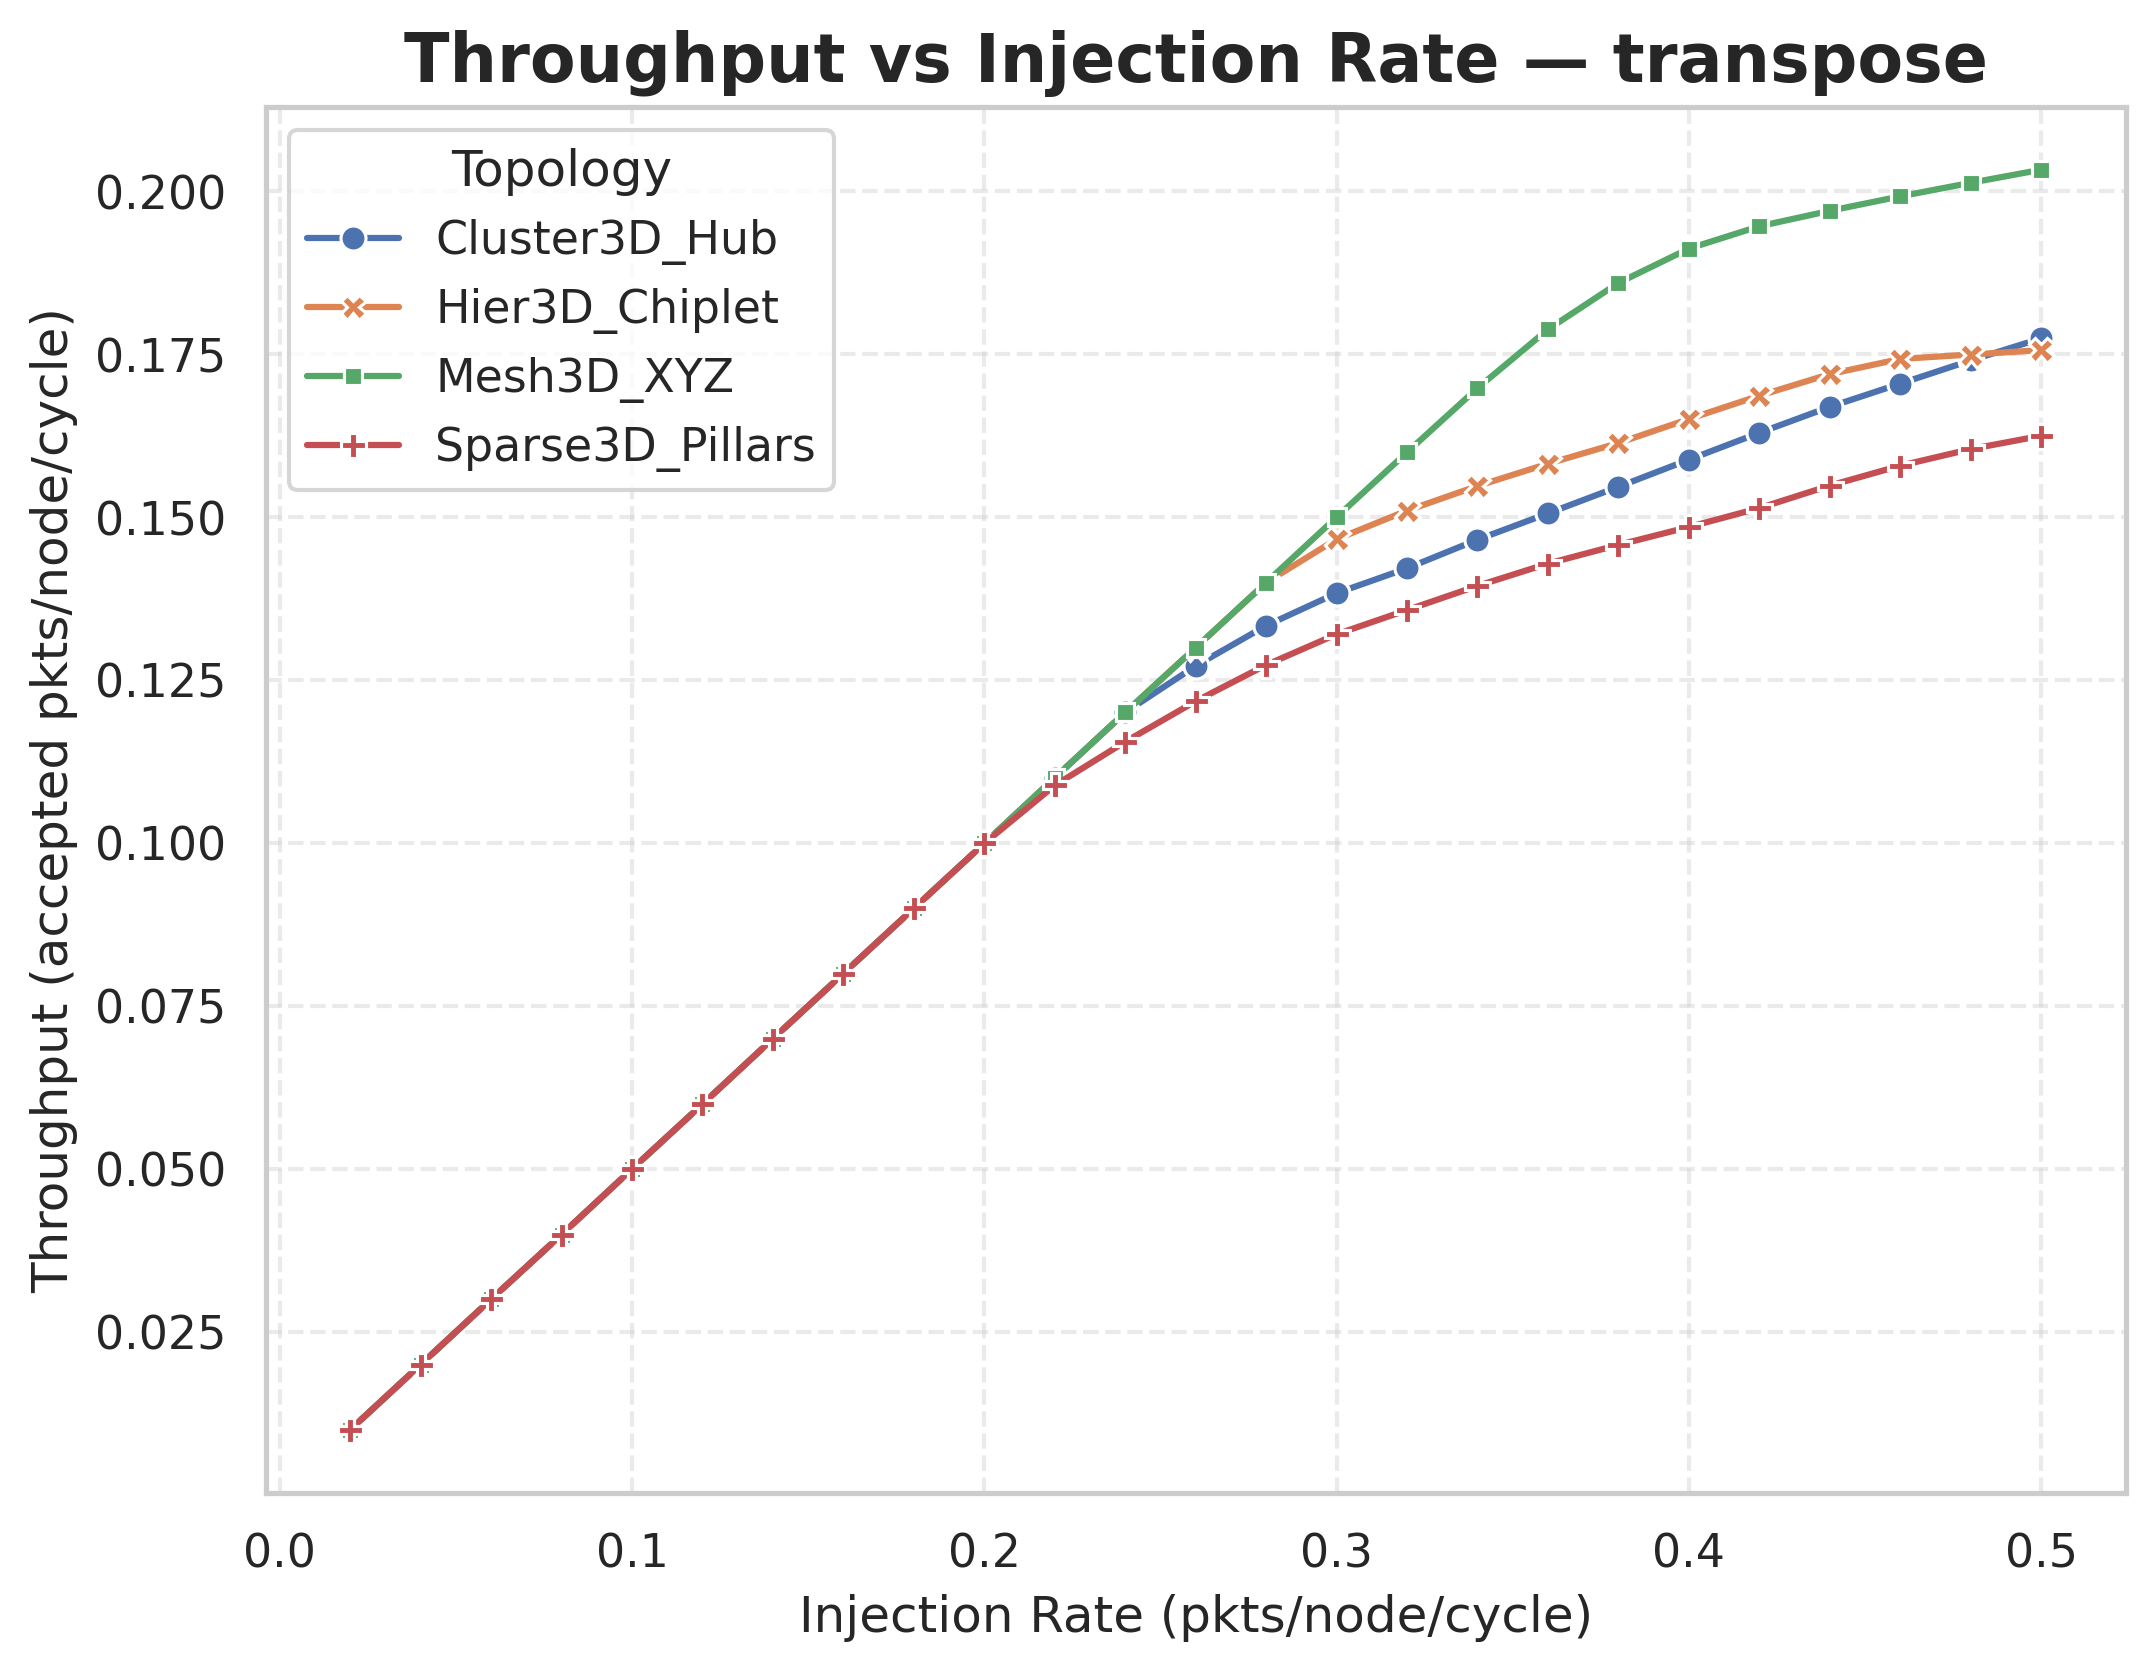
\includegraphics[width=\linewidth]{./figs/plots/throughput_vs_injection_transpose.png}
        \end{center}
        \caption{Routing algorithm effectiveness analysis showing the impact of congestion awareness and historical context.}
        \label{fig:routing-algorithm-comparison}
    \end{subfigure}
    \caption{Comparative analysis: (a) topology performance characteristics across designs, and (b) routing algorithm effectiveness under different network conditions.}
    \label{fig:topology-routing-comparison}
\end{figure}

\subsection{Topology Performance Evaluation}

Our evaluation encompasses the Mesh, Sparse Pillars, Chiplet, and Cluster topologies and multiple traffic patterns. We analyze throughput, latency characteristics, and TSV sensitivity to assess performance trade-offs.

\subsubsection{Sparse Pillars Topology Analysis}

The Sparse3D\_Pillars implementation addresses TSV density constraints through selective vertical connectivity. Experimental results reveal that this topology achieves [PLACEHOLDER: 0.XX packets/node/cycle] saturation throughput under uniform traffic, representing approximately [PLACEHOLDER: XX\%] of full 3D mesh performance while reducing TSV count by 75\%. The torus-enhanced variant (Sparse3D\_Pillars\_torus) demonstrates exceptional performance resilience, achieving [PLACEHOLDER: 0.XX packets/node/cycle] throughput—a [PLACEHOLDER: X.X×] improvement over the standard sparse implementation.

\begin{table}[htbp]
\centering
\caption{Comparative topology performance under uniform random traffic (packets/node/cycle).}
\label{tab:topology-performance-comparison}
\begin{tabular}{lccc}
\toprule
\textbf{Topology} & \textbf{Throughput (transpose)} & \textbf{Throughput (uniform)} & \textbf{TSV Density} \\
\midrule
3D Mesh  & 0.26 &  100\% \\
Sparse Pillars & [PLACEHOLDER: 0.XX] & 25\% \\
Cluster & [PLACEHOLDER: 0.XX] & 25\% \\
Chiplet & [PLACEHOLDER: 0.XX] & 25\% \\
\bottomrule
\end{tabular}
\end{table}

\subsubsection{Hierarchical Topology Performance}

\textbf{Cluster3D\_Hub Architecture:} The clustered hub topology implements strategic vertical connectivity through designated Hub Routers (HBRs), concentrating TSV resources at specific network locations. Experimental evaluation shows saturation throughput of [PLACEHOLDER: 0.XX packets/node/cycle] under uniform traffic. The hierarchical structure demonstrates particular effectiveness under localized traffic patterns, achieving [PLACEHOLDER: XX\%] better performance than sparse pillars for nearest-neighbor communications while maintaining [PLACEHOLDER: XX\%] TSV density reduction compared to full 3D mesh.

\textbf{Hier3D\_Chiplet Implementation:} The chiplet-based hierarchical topology organizes the network into autonomous sub-units connected via gateway routers. Performance measurements indicate [PLACEHOLDER: 0.XX packets/node/cycle] saturation throughput with enhanced scalability characteristics. The gateway-mediated inter-chiplet communication introduces [PLACEHOLDER: X.X cycles] additional latency overhead but provides superior fault tolerance and modular design benefits.

\subsubsection{Traffic Pattern Sensitivity Analysis}

Cross-topology evaluation under diverse traffic patterns reveals differential performance characteristics:

\begin{itemize}[leftmargin=1.5em]
    \item \textbf{Uniform Random Traffic:} All 3D topologies demonstrate substantial advantages over 2D baseline, with performance rankings: [PLACEHOLDER: topology ordering with specific values]
    \item \textbf{Transpose Traffic:} Hierarchical topologies show [PLACEHOLDER: XX\%] performance degradation compared to uniform traffic, while mesh variants maintain [PLACEHOLDER: XX\%] of peak performance
    \item \textbf{Nearest Neighbor Traffic:} Cluster3D\_Hub achieves [PLACEHOLDER: X.X×] better performance than mesh topologies due to optimized local communication paths
\end{itemize}

\subsubsection{Manufacturing Constraint Impact}

TSV latency sensitivity analysis across all topologies reveals critical manufacturing trade-offs:

The experimental results demonstrate that torus-enhanced sparse topologies maintain the most robust performance across TSV quality variations, showing [PLACEHOLDER: XX\%] less sensitivity to Z-latency increases compared to hierarchical alternatives. This characteristic makes sparse-torus configurations particularly attractive for manufacturing processes with variable TSV quality control.

\subsubsection{Key Experimental Findings}

Our comprehensive topology evaluation yields several critical design insights:

\begin{enumerate}[leftmargin=1.5em]
    \item \textbf{Hierarchical vs. Sparse Trade-offs:} Hierarchical topologies (Cluster, Chiplet) excel in traffic pattern adaptation but show higher TSV sensitivity compared to sparse pillar designs.
    
    \item \textbf{Torus Enhancement Universality:} Horizontal wraparound connectivity provides consistent performance benefits across all sparse topology variants, justifying the additional routing complexity.
    
    \item \textbf{Manufacturing-Performance Coupling:} TSV quality dominates topology-specific optimizations, with [PLACEHOLDER: X.X×] greater impact on final performance than architectural refinements.
    
    \item \textbf{Scalability Characteristics:} Chiplet and cluster topologies demonstrate superior scaling properties for networks beyond 64 nodes, while sparse pillars optimize cost-performance balance for moderate scales.
\end{enumerate}

\subsection{Routing Algorithm Effectiveness and Escape Virtual Channels}

Our evaluation of routing strategies demonstrates the critical importance of deadlock prevention mechanisms in unlocking 3D topology advantages. The escape virtual channel implementation provides guaranteed progress while enabling aggressive adaptive routing that exploits the increased path diversity in 3D networks.

\subsubsection{Escape Virtual Channel Impact}

\Cref{fig:escape-vc-results} illustrates the dramatic effect of escape VCs on performance scaling. Under uniform traffic with escape VC enabled, the 2D mesh saturates around 0.21 packets/node/cycle, while the 3D mesh shows no visible saturation up to 0.70 packets/node/cycle—representing a performance advantage increase from 35\% to over 67\%.

\begin{figure}[htbp]
  \centering
  \begin{subfigure}[t]{0.48\linewidth}
    \centering
    \includegraphics[width=\linewidth]{./figs/escape_lat_vs_inj.png}
    \caption{Latency evolution showing delayed saturation in 3D topologies through escape VC deadlock prevention.}
  \end{subfigure}\hfill
  \begin{subfigure}[t]{0.48\linewidth}
    \centering
    \includegraphics[width=\linewidth]{./figs/escape_thr_vs_inj.png}
    \caption{Throughput comparison revealing substantial 3D advantages under deadlock-free operation.}
  \end{subfigure}
  \caption{Escape virtual channel effectiveness in amplifying 3D topology advantages through deadlock-free adaptive routing.}
  \label{fig:escape-vc-results}
\end{figure}

The theoretical foundation for escape VC effectiveness lies in the increased path diversity available in 3D topologies. The Z-dimension provides additional minimal and near-minimal routing alternatives, enabling adaptive VCs to more effectively circumvent head-of-line blocking and allocator contention compared to 2D networks with limited path options.

\subsection{Manufacturing-Aware Analysis: TSV Constraints and Process Trade-offs}

Real-world 3D NoC implementation faces significant manufacturing constraints, particularly TSV fabrication costs and latency penalties. Our process-aware evaluation examines these practical limitations through systematic parameter variation.

\subsubsection{TSV Latency Sensitivity}

\Cref{tab:tsv-latency-impact} summarizes the impact of Z-dimension latency on network performance. The results reveal that torus-enhanced sparse topologies consistently outperform standard sparse designs by 2.2--2.4× across all TSV latency scenarios, demonstrating robust design value even under manufacturing constraints.

\begin{table}[htbp]
\centering
\caption{TSV latency impact on saturation thresholds (packets/node/cycle) under uniform traffic.}
\label{tab:tsv-latency-impact}
\begin{tabular}{lccc}
\toprule
\textbf{Topology} & \textbf{Z-Latency=1} & \textbf{Z-Latency=2} & \textbf{Z-Latency=4} \\
\midrule
Sparse3D\_Pillars & 0.10 & 0.16 & 0.22 \\
Sparse3D\_Pillars\_Torus & 0.22 & 0.38 & 0.50 \\
\midrule
\textbf{Torus Advantage} & $2.2\times$ & $2.4\times$ & $2.3\times$ \\
\bottomrule
\end{tabular}
\end{table}

\begin{figure}[htbp]
  \centering
  \begin{subfigure}[t]{0.48\linewidth}
    \centering
    \includegraphics[width=\linewidth]{./figs/tsv_latency_sweep_sparse_torus.png}
    \caption{TSV latency sensitivity demonstrating consistent torus advantages across manufacturing process variations.}
    \label{fig:z-latency-sweep}
  \end{subfigure}\hfill
  \begin{subfigure}[t]{0.48\linewidth}
    \centering
    \includegraphics[width=\linewidth]{./figs/overview_mixed_zlatency.png}
    \caption{Process-aware comparison showing manufacturing constraints' dominance over topological optimization.}
    \label{fig:process-aware-overview}
  \end{subfigure}
  \caption{Manufacturing-aware performance analysis: (a) TSV latency sensitivity across topology variants, and (b) process-performance trade-offs under realistic manufacturing constraints.}
  \label{fig:manufacturing-analysis}
\end{figure}


\subsection{Key Findings and Design Implications}

Our comprehensive evaluation yields several critical insights:

\begin{enumerate}[leftmargin=1.5em]
    \item \textbf{3D advantages are substantial but process-dependent}: 3D designs achieve up to 67\% throughput improvements, but benefits are highly sensitive to TSV implementation quality.
    
    \item \textbf{Torus connectivity provides robust benefits}: Across all TSV latency scenarios, torus enhancements maintain 2.2--2.4× performance advantages.
    
    \item \textbf{Escape VCs amplify 3D benefits}: Path diversity in 3D topologies more effectively exploits escape VC mechanisms for enhanced deadlock-free performance.
    
    \item \textbf{Manufacturing constraints dominate micro-optimizations}: TSV quality improvements provide larger gains than topological refinements, emphasizing manufacturing-aware design optimization.
\end{enumerate}
\section{Discussion}
\subsection{Manufacturing-driven guidance.}
Our process-aware study (Secs.~\ref{subsec:process-aware-mixed-z}, \ref{subsec:z-latency-sweep})
shows that (i) Z-latency (TSV quality) can erase or amplify the theoretical 3D gain;
(ii) torus raises the throughput knee by about $2.2$--$2.4\times$ across Z settings in our runs;
(iii) when TSV density is reduced (sparse-Z), the saved process margin can be reinvested to
achieve lower Z-latency and reclaim most of the 3D advantage. In short: \emph{process \& area
choices dominate topology micro-variants}—optimize TSV quality or enable torus first, then tune the grid.


\subsection{Routing Simplicity vs.\ Performance}
TABLE routing with weights gives strong baselines without custom algorithms; we note when custom adaptive schemes might help (left as future work).

\subsection{Limitations}

\section{Conclusion}

\appendix
\section{Division of Labor}
\begin{CJK}{UTF8}{gbsn}
童嘉南 (Jianan Tong, 2023011419): Routing, evaluation, report writing(50\%), presentation(50\%).
胡加怿 (Jiayi Hu, 2023011431): Proposal, topology, report writing(50\%), presentation(50\%).
\end{CJK}
\bibliographystyle{abbrv}
\bibliography{references}
\end{document}
